\documentclass[landscape,a4paper]{extarticle}
\usepackage{caption}
\usepackage{multicol}
\usepackage[top=1em,bottom=1em,left=1em,right=1em]{geometry}
\usepackage[framemethod=tikz]{mdframed}
\usepackage{microtype}
\usepackage{pdfpages}
\usepackage{amsmath, amssymb, amsthm}
\usepackage{anyfontsize}
\usepackage[shortlabels]{enumitem}
\usepackage{graphicx, float}
\usepackage{ulem} % Using \uline{} instead of \underline{} will make the line closer to the word
\usepackage{xcolor}
\usepackage{tgschola}

\let\bar\overline

% Remove vertical space before and after all verbatim environments
\BeforeBeginEnvironment{verbatim}{\vspace{-\topsep}\vspace{-\partopsep}}
\AfterEndEnvironment{verbatim}{\vspace{-\topsep}\vspace{-\partopsep}}

% Configure image directory
\graphicspath{{images/}}

\newenvironment{Figure}
  {\par\noindent\minipage{\linewidth}}
  {\endminipage\par\medskip}
  
% Remove caption labels
\captionsetup{labelformat=empty,labelsep=none}

% No paragraph indent
\setlength{\parindent}{0pt}

% No spaces between list items, no left margins
\setlist[enumerate]{nosep, leftmargin=*}
\setlist[itemize]{nosep, leftmargin=*}

% No spaces before and after math mode
\expandafter\def\expandafter\normalsize\expandafter{%
    \normalsize%
    \setlength\abovedisplayskip{0pt}%
    \setlength\belowdisplayskip{0pt}%
    \setlength\abovedisplayshortskip{-8pt}%
    \setlength\belowdisplayshortskip{2pt}%
}

\begin{document}
\fontsize{7}{8}\selectfont
\fontfamily{qcs}\selectfont
\begin{multicols*}{5}
    \uline{\textbf{Lecture 3 - Requirements}}

    Requirements are a set of capabilities and constraints

    [IEEE]
    \begin{enumerate}
        \item A condition or capability needed by a user to solve a problem or achieve an objective
        \item A condition or capability that must be met or possessed by a system or system component to satisfy a contract, standard, specification, or other formally imposed documents
        \item A documented representation fo a condition or capability as in (1) or (2)
    \end{enumerate}
    \textbf{Example of capability:} system should allow a requester to specify pick-up and drop-off locations.
    \textbf{Example of constraint:} pick-up and drop-off locations should be from a list of on-campus buildings / landmarks.

    \textbf{Requirements Development Phases}
    \begin{Figure}
        \centering
        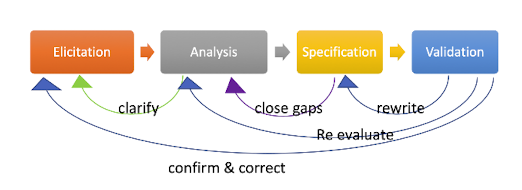
\includegraphics[width=\linewidth]{requirements_development_phases.png}
    \end{Figure}
    \textbf{Elicitation}: Discover requirements (through interview, workshop, document analysis, prototyping)

    \textbf{Analysis}: Analyze, decompose, derive, understand, negotiate requirements, identify gaps

    \textbf{Specification}: Written and illustrated requirements for comprehension, review, and use

    \textbf{Validation}: Confirm correct set of requirements that will enable developers to build a solution

    \textbf{Sources of software requirements}
    \begin{itemize}
        \item Documents
        \begin{itemize}
            \item Descriptions of current or competing products
            \item Standards or regulations
            \item help desk problem reports
        \end{itemize}
        \item Interviews
        \begin{itemize}
            \item Focus groups
            \item Use case workshops
            \item Product champions as key customer rep
        \end{itemize}
        \item Questionnaires and marketing surveys
        \begin{itemize}
            \item Run a pilot first - difficult to ask clear questions
        \end{itemize}
        \item Event-response tables
        \begin{itemize}
            \item Identify external stimuli and describe system responses
        \end{itemize}
        \item Observation - watch users do their jobs
        \begin{itemize}
            \item Create workflow diagrams
            \item "Day in the life" studies
            \item Look at what information the user has when performing a particular task
        \end{itemize}
        \item Prototyping
        \begin{itemize}
            \item Useful for requirements, design, and implementation
        \end{itemize}
    \end{itemize}
    \textbf{FR vs NFR}

    \textbf{FR} describes something the system should do
    \begin{itemize}
        \item specify a behavior or function
        \item e.g. the passenger shall be able to print boarding passes for all flight segments for which she has checked in
    \end{itemize}
    \textbf{NFR} describes something not directly related to the functionality of the system
    \begin{itemize}
        \item May describe how well the system works
        \item Can include other attributes too (e.g. reliability, efficiency, usability)
        \item E.g. mean time between failure $\geq$ 9000 hrs
    \end{itemize}

    \textbf{External vs Internal Quality Attributes}

    \textbf{External:}

    \begin{itemize}
        \item Observed when the software is executing
        \item Impacts user's experienece of using the software
        \item Develops the user's perception of software quality
        \item E.g. Availability, performace, robustness, safety, security, reliability, deployability, compatibility, installability, usability, interoperability, integrity
    \end{itemize}

    \textbf{Internal:}

    \begin{itemize}
        \item Not directly observed when software is executing
        \item Perceived by the developers and maintainers
        \item Encompasses aspects of design that may impact external attributes
        \item E.g. Scalability, efficiency, modifiability, verifiability, portability, maintainability, reusability, testability
    \end{itemize}
    % \begin{Figure}
    %     \centering

    %     % If the image is too wide, use a smaller fraction, e.g. 0.8\linewidth.
    %     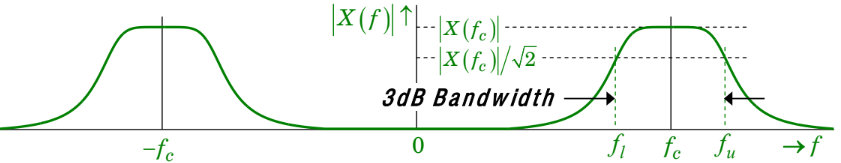
\includegraphics[width=\linewidth]{sample_image.png}
    % \end{Figure}
\end{multicols*}
\end{document}